\documentclass{article}
\usepackage{ctex}
\usepackage{amsmath}
\usepackage{amssymb}
\usepackage{mathtools}
\usepackage{graphicx}
\usepackage{booktabs}
\usepackage{fancyhdr}
\usepackage{pgfplots}
\fancyhf{}
\lhead{《电子电路与系统基础实验》}
\chead{2025年}
\rhead{第二次实验}
\pagestyle{fancy}
\begin{document}
\begin{titlepage}
    \centering
    
    % 标题
    \vspace*{1cm}
    \Huge
    \textbf{实验题目:} 心电信号检测电路的搭建和测试
    
    % 空白行
    \vspace{8cm}
    
    % 各种信息
    \large
    \textbf{班级:} 丁健 \\
    \textbf{学号:} 2023013384 \\
    \textbf{姓名:} 为先32 \\ 
    \textbf{日期:} \today

\end{titlepage}
\section{实验目的}
\begin{enumerate}
    \item 掌握数字存储示波器和函数信号发生器的正确调整方法
    \item 结合常用电子仪器的使用,掌握常用电路参数(输入电阻、输出电阻、增益、幅频特性等)的测量方法。
    \item 通过实验直观理解放大器、滤波器等单元的功用,并利用已有模块,组建调试,在示波器上显示自己的心电信号,着重构建系统设计的概念,培养学生对于电子工程和生物医学工程的兴趣。
\end{enumerate}

\section{实验数据整理与分析}
\subsection{正弦小信号确定差分放大器的差模增益}
如图所示:
\begin{figure}[htbp]
    \centering
    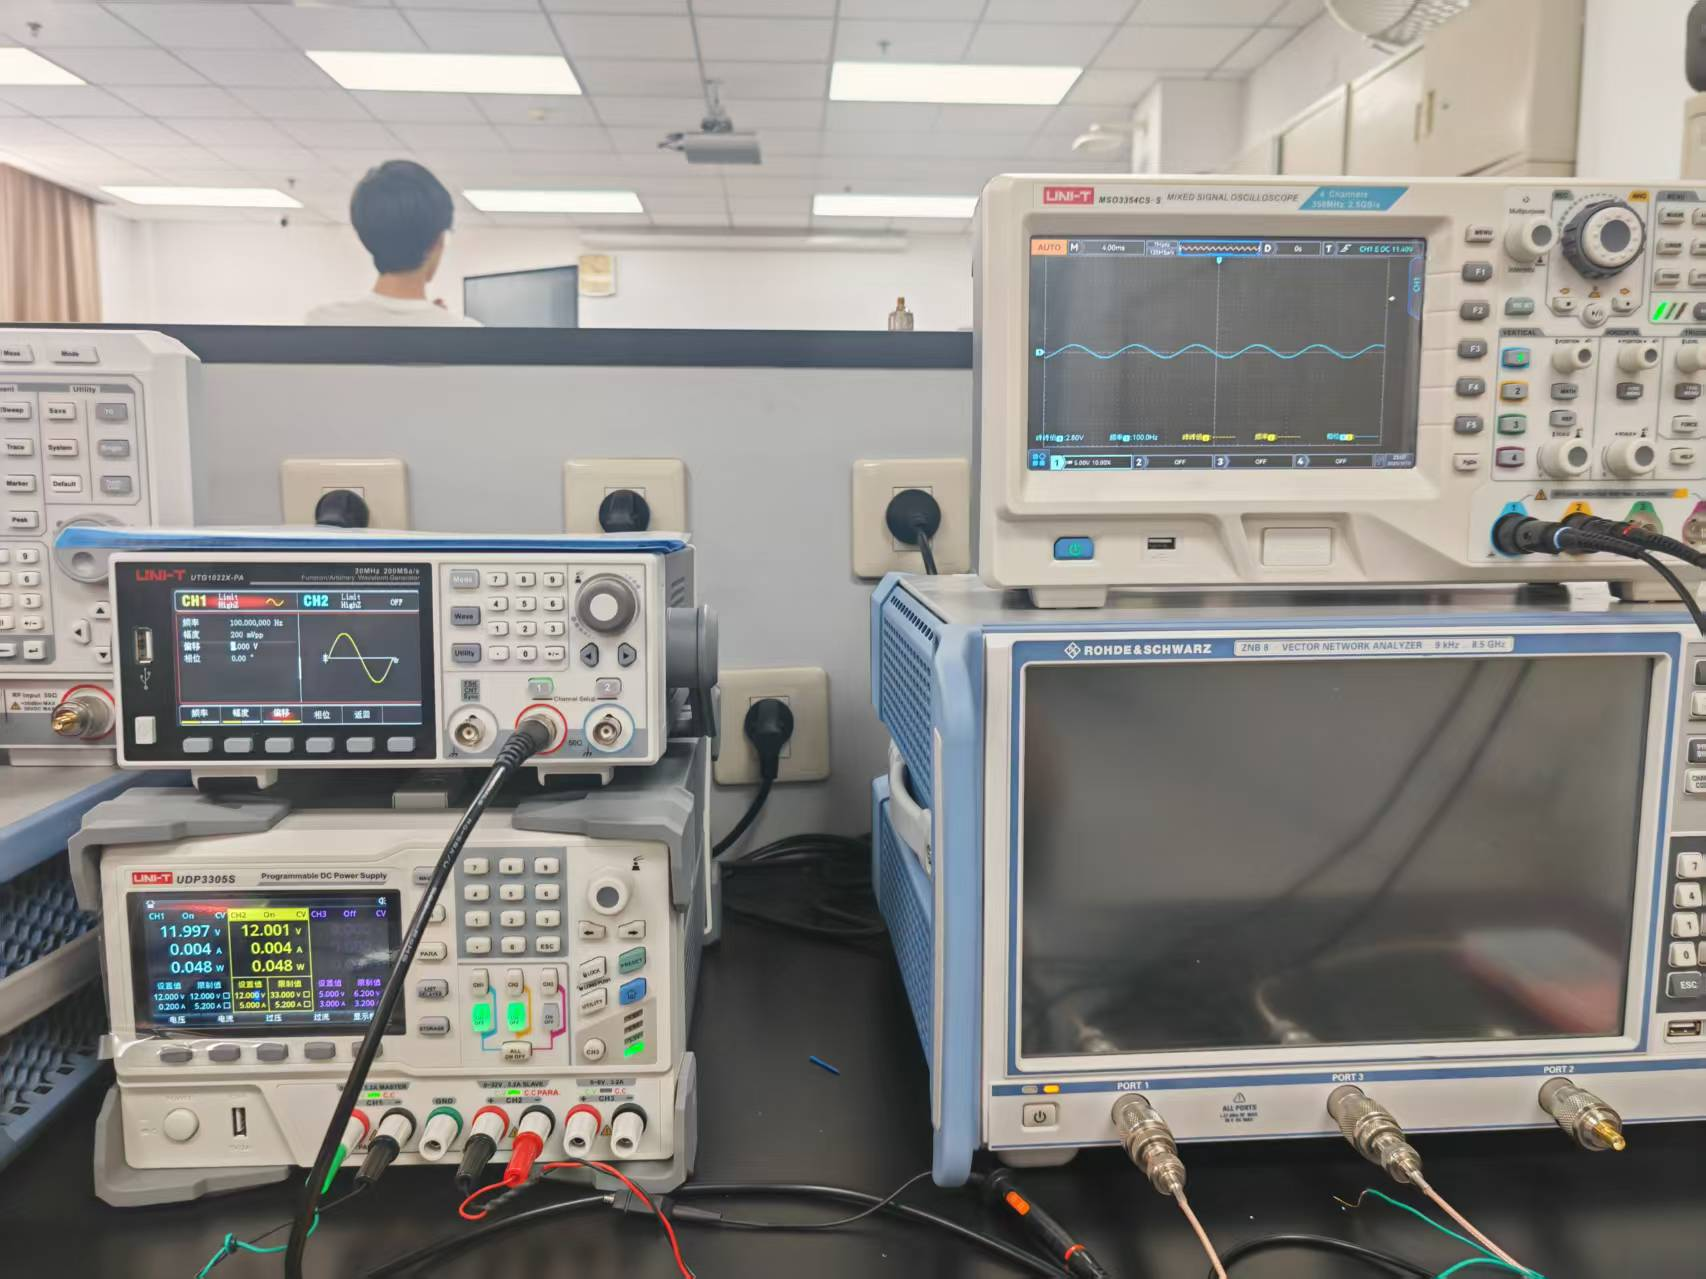
\includegraphics[width=300pt,height=200pt]{zengda.jpg}
\end{figure}
输入正弦电压峰峰值为200mVpp,示波器显示输出端峰峰值为2.80V,差模增益为$\frac{2.8V}{200mV} = 14$倍。
\subsection{测量高通滤波器的输出波形}
输入信号为200mV,周期为5s的方波信号,测量高通滤波器的输出波形,即阶跃响应\\
如图所示:
\begin{figure}[htbp]
    \centering
    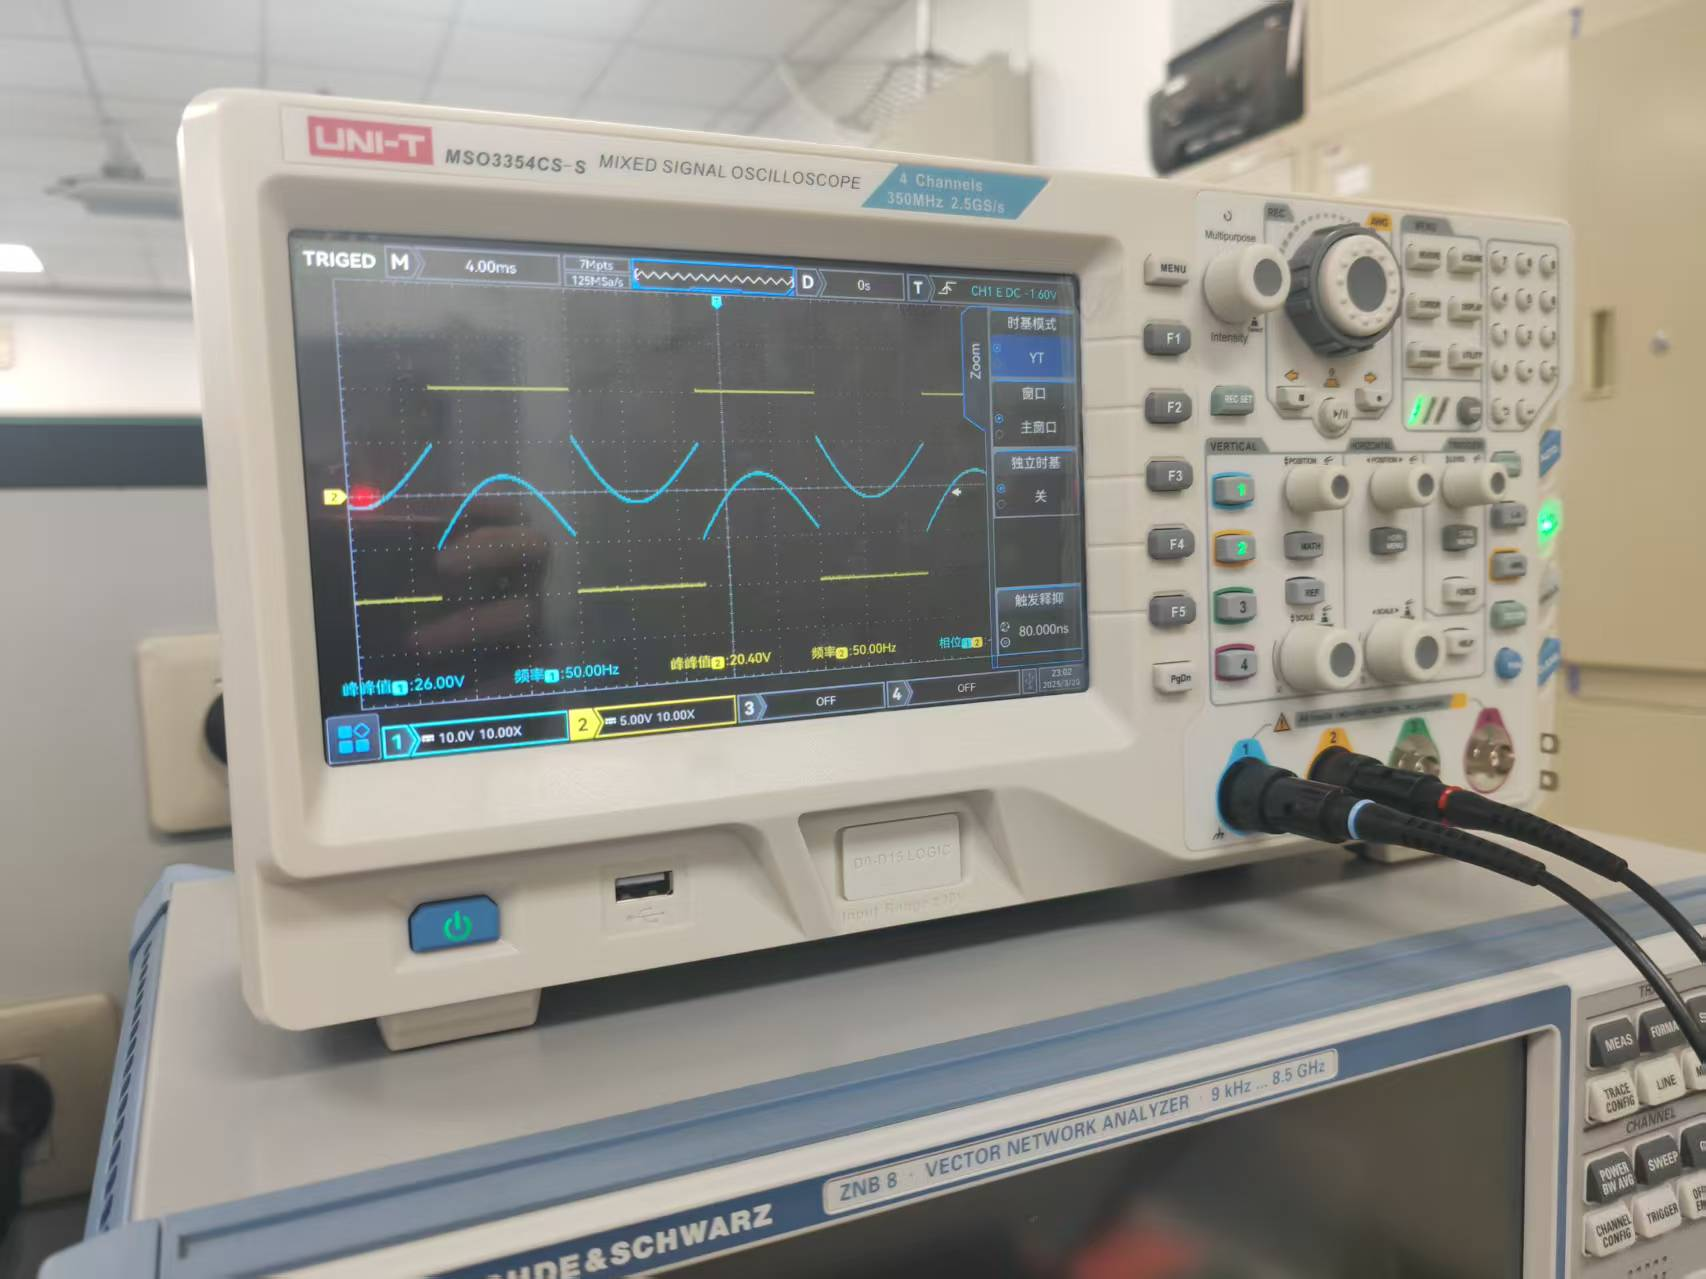
\includegraphics[width=300pt,height=200pt]{bobo.jpg}
\end{figure}

\subsection{低通滤波器的幅频特性}
幅频特性记录记录如图所示:
\begin{figure}
    \centering
    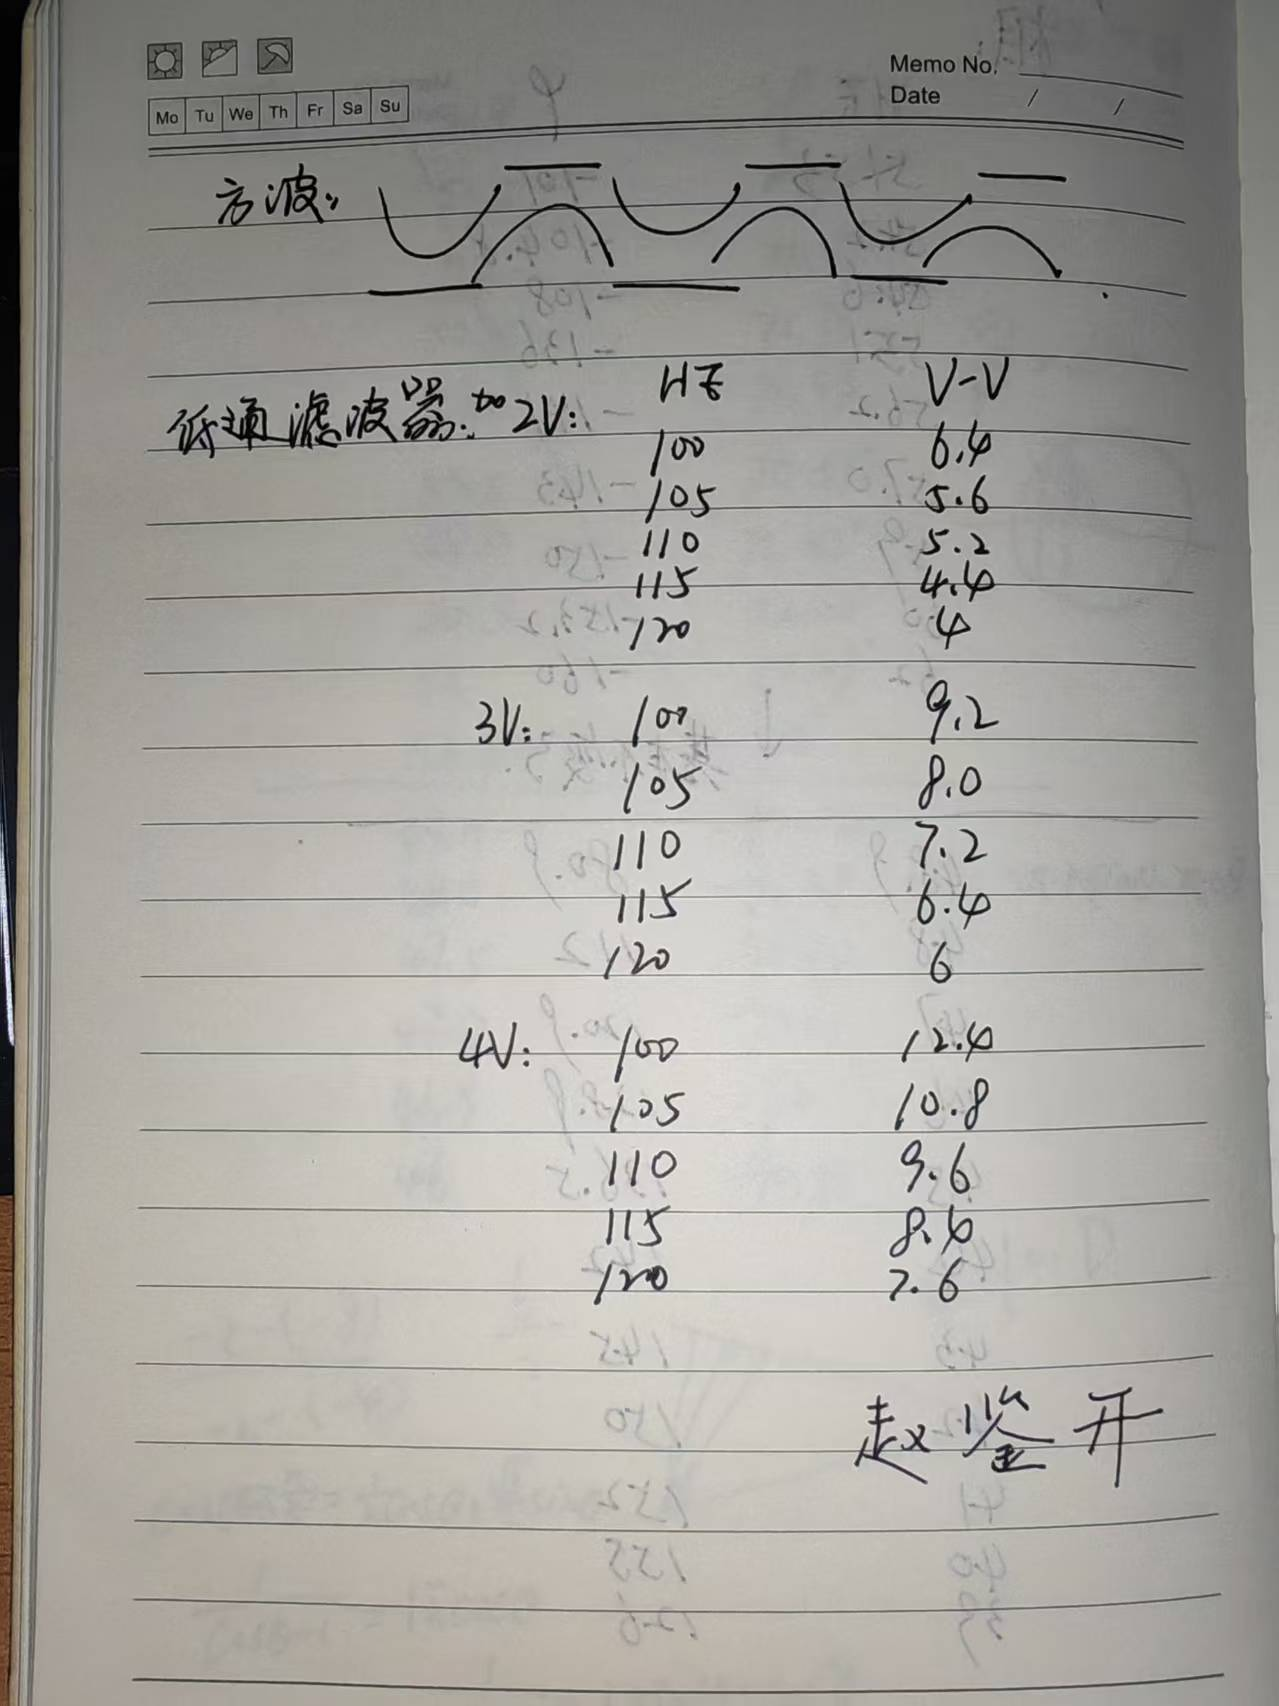
\includegraphics[width=300pt,height=350pt]{ditong.jpg}
\end{figure}

\begin{table}[h!]
    \centering
    \caption{低通滤波器的幅频特性}
    \label{tab:example}

    \begin{tabular}{ccc}
    \hline 
    % 表头
    输入电压(V) & 频率(Hz) & 输出峰峰值(V-V) \\ 
    2 & 100 & 6.4 \\ 
    2 & 105 & 5.6 \\ 
    2 & 110 & 5.2 \\ 
    2 & 115 & 4.4 \\ 
    2 & 120 & 4 \\ 
    3 & 100 & 9.2 \\ 
    3 & 105 & 8.0 \\ 
    3 & 110 & 7.2 \\ 
    3 & 115 & 6.4 \\ 
    3 & 120 & 6 \\ 
    4 & 100 & 12.4 \\ 
    4 & 105 & 10.8 \\ 
    4 & 110 & 9.6 \\ 
    4 & 115 & 8.4 \\ 
    4 & 120 & 7.6 \\ 
\end{tabular}
    
    \end{table}

    \begin{tikzpicture}
        \begin{axis}[
            title=低通滤波器的幅频特性,
            xlabel=频率(HZ),
            ylabel=输出峰峰值,
            legend pos=north west
        ]
        % 直接从表格数据绘制
        \addplot table {
            x   y
            100  6.4 
            105  5.6 
            110  5.2 
            115  4.4  
            120  4  
        };
        \addlegendentry{$V_\text{in}$ = 2V}

        \addplot table {
            x   y
            100  9.2 
            105  8.0 
            110  7.2 
            115  6.4  
            120  6
        };
        \addlegendentry{$V_\text{in}$ = 3V}

        \addplot table {
            x   y
            100  12.4 
            105  10.8
            110  9.6 
            115  8.4  
            120  7.6
        };
        \addlegendentry{$V_\text{in}$ = 4V}
        
        % 或者引用外部数据文件
        % \addplot table {datafile.dat};
        \end{axis}
        \end{tikzpicture}
    
        低通滤波器的阶跃响应:
        \begin{figure}[htbp]
            \centering
            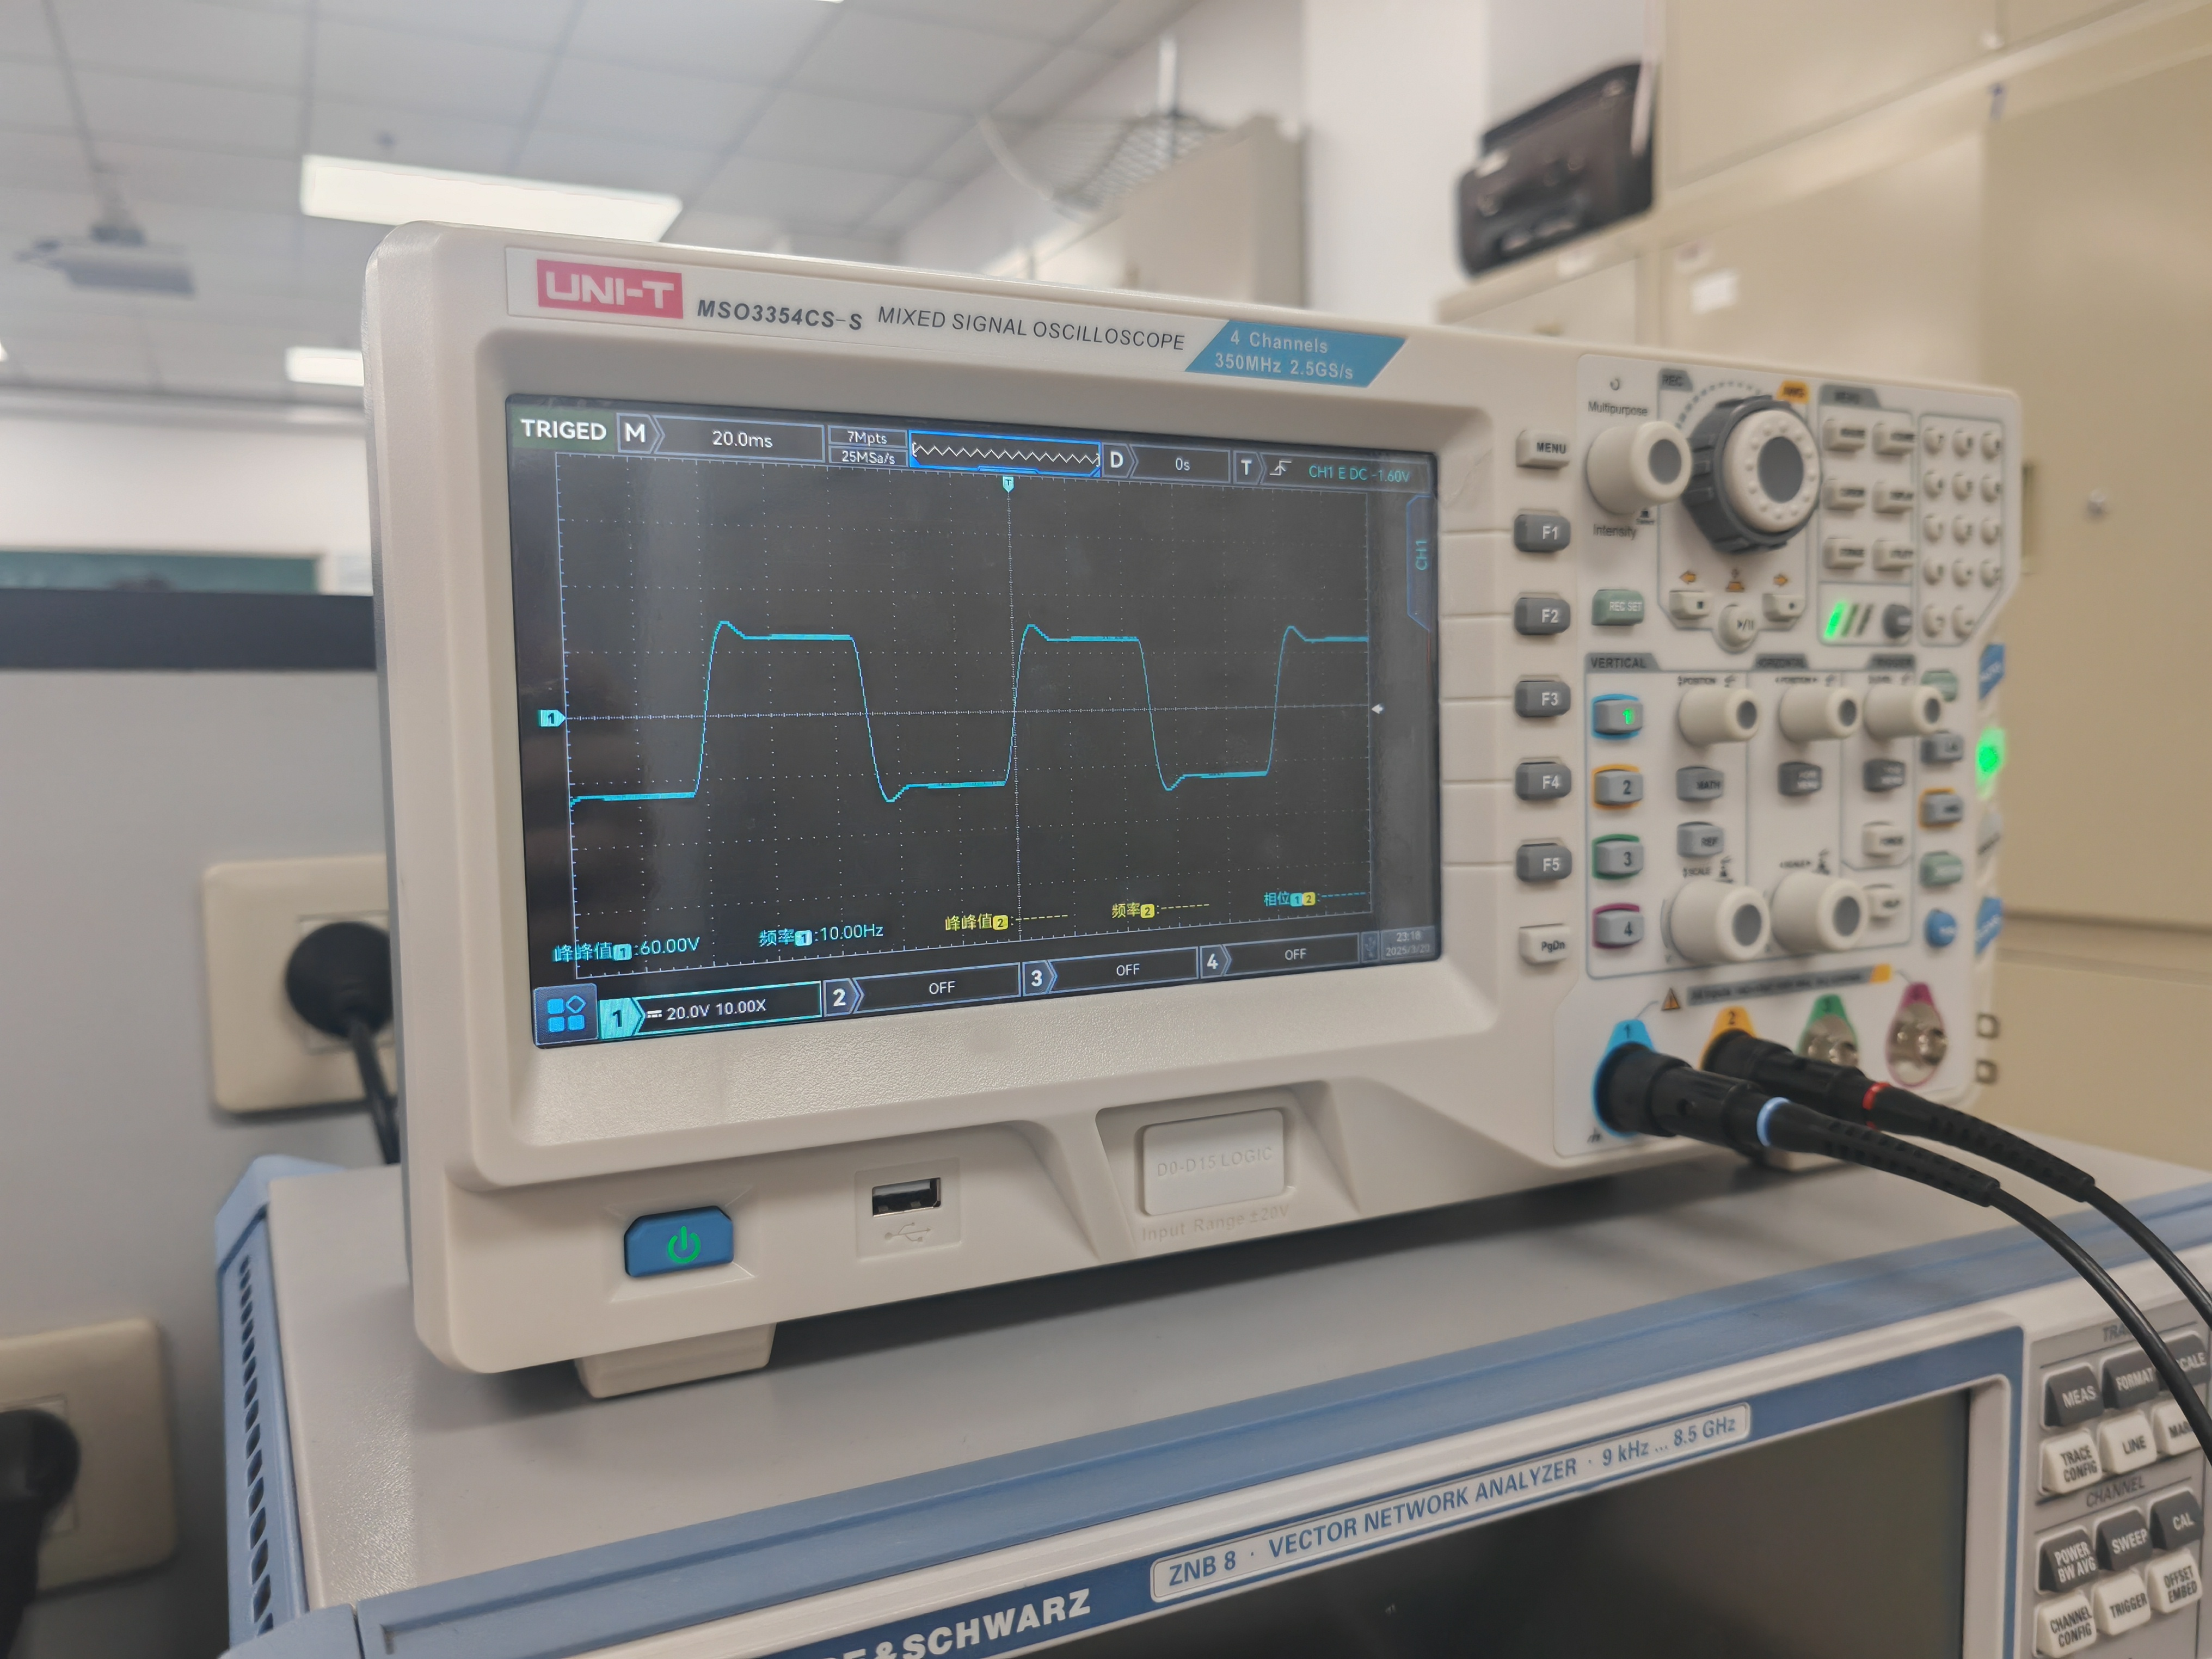
\includegraphics[width=200pt,height=180pt]{1.jpg}
            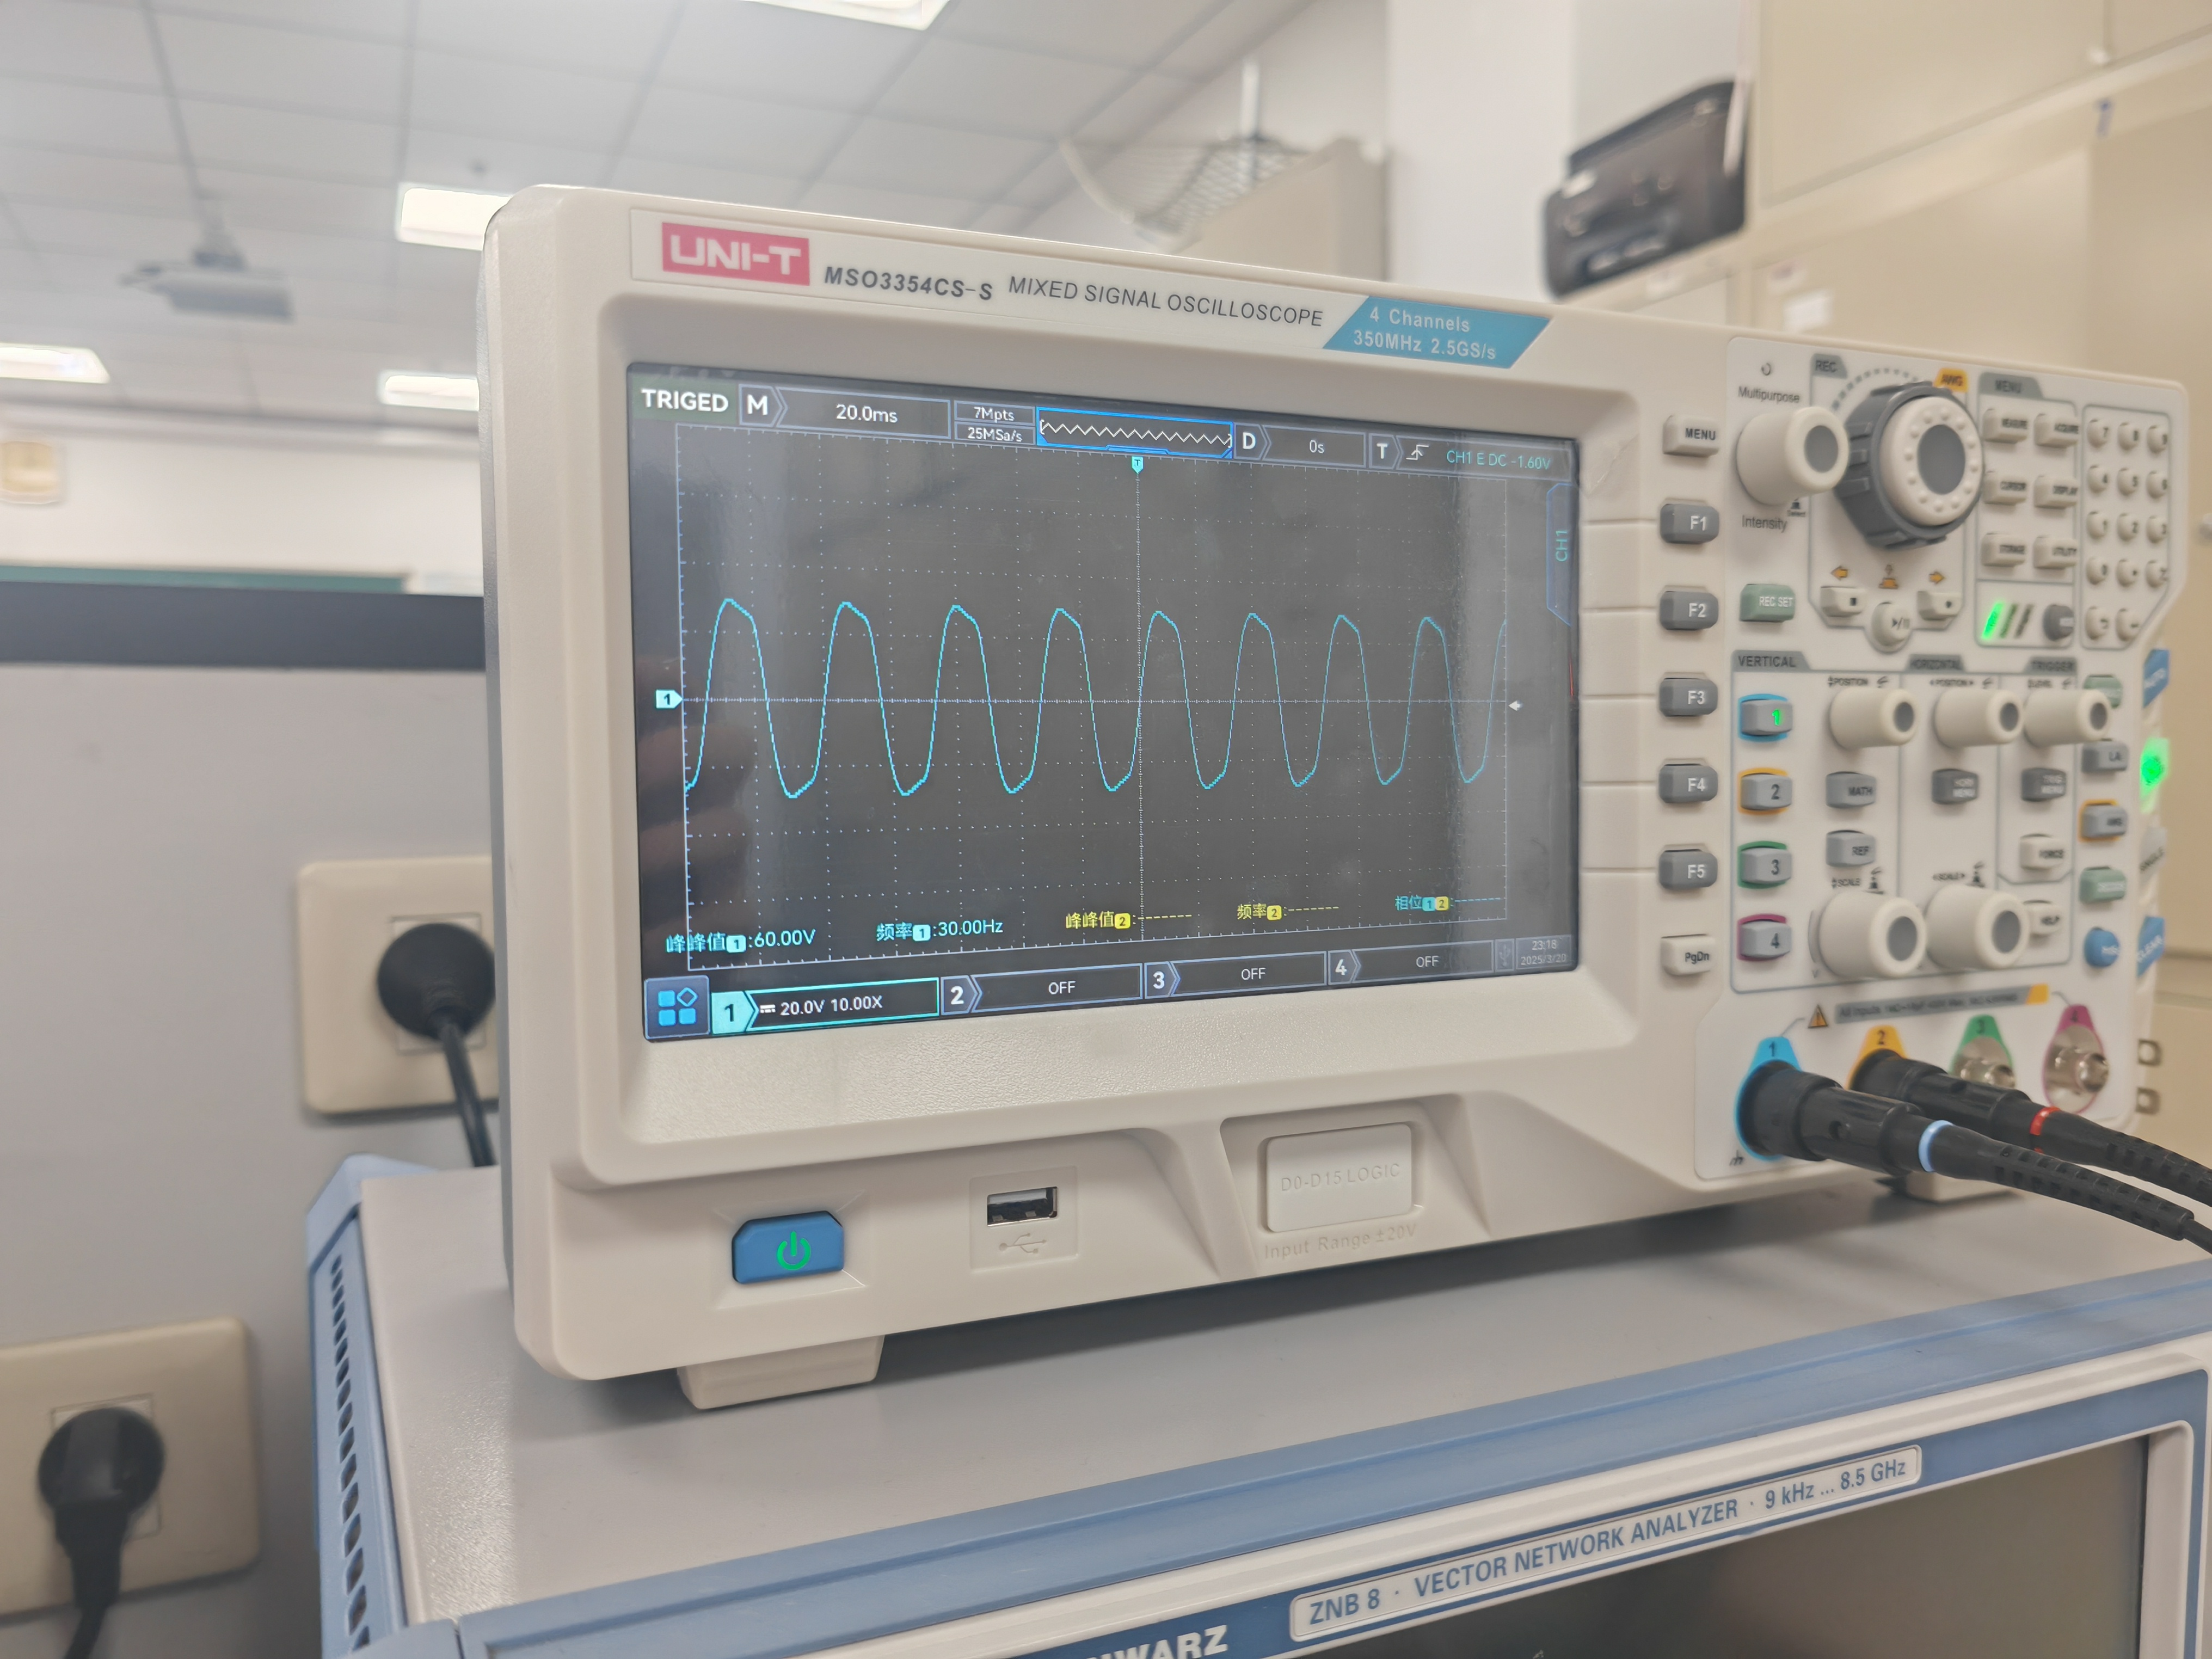
\includegraphics[width=200pt,height=180pt]{2.jpg}
            \caption{低通滤波器的阶跃响应}
        \end{figure}

\subsection{调节50Hz陷波器,并测量50Hz陷波器在50Hz附近的幅频和相频特性}

幅频特性记录如图:
\begin{figure}[htbp]
    \centering
    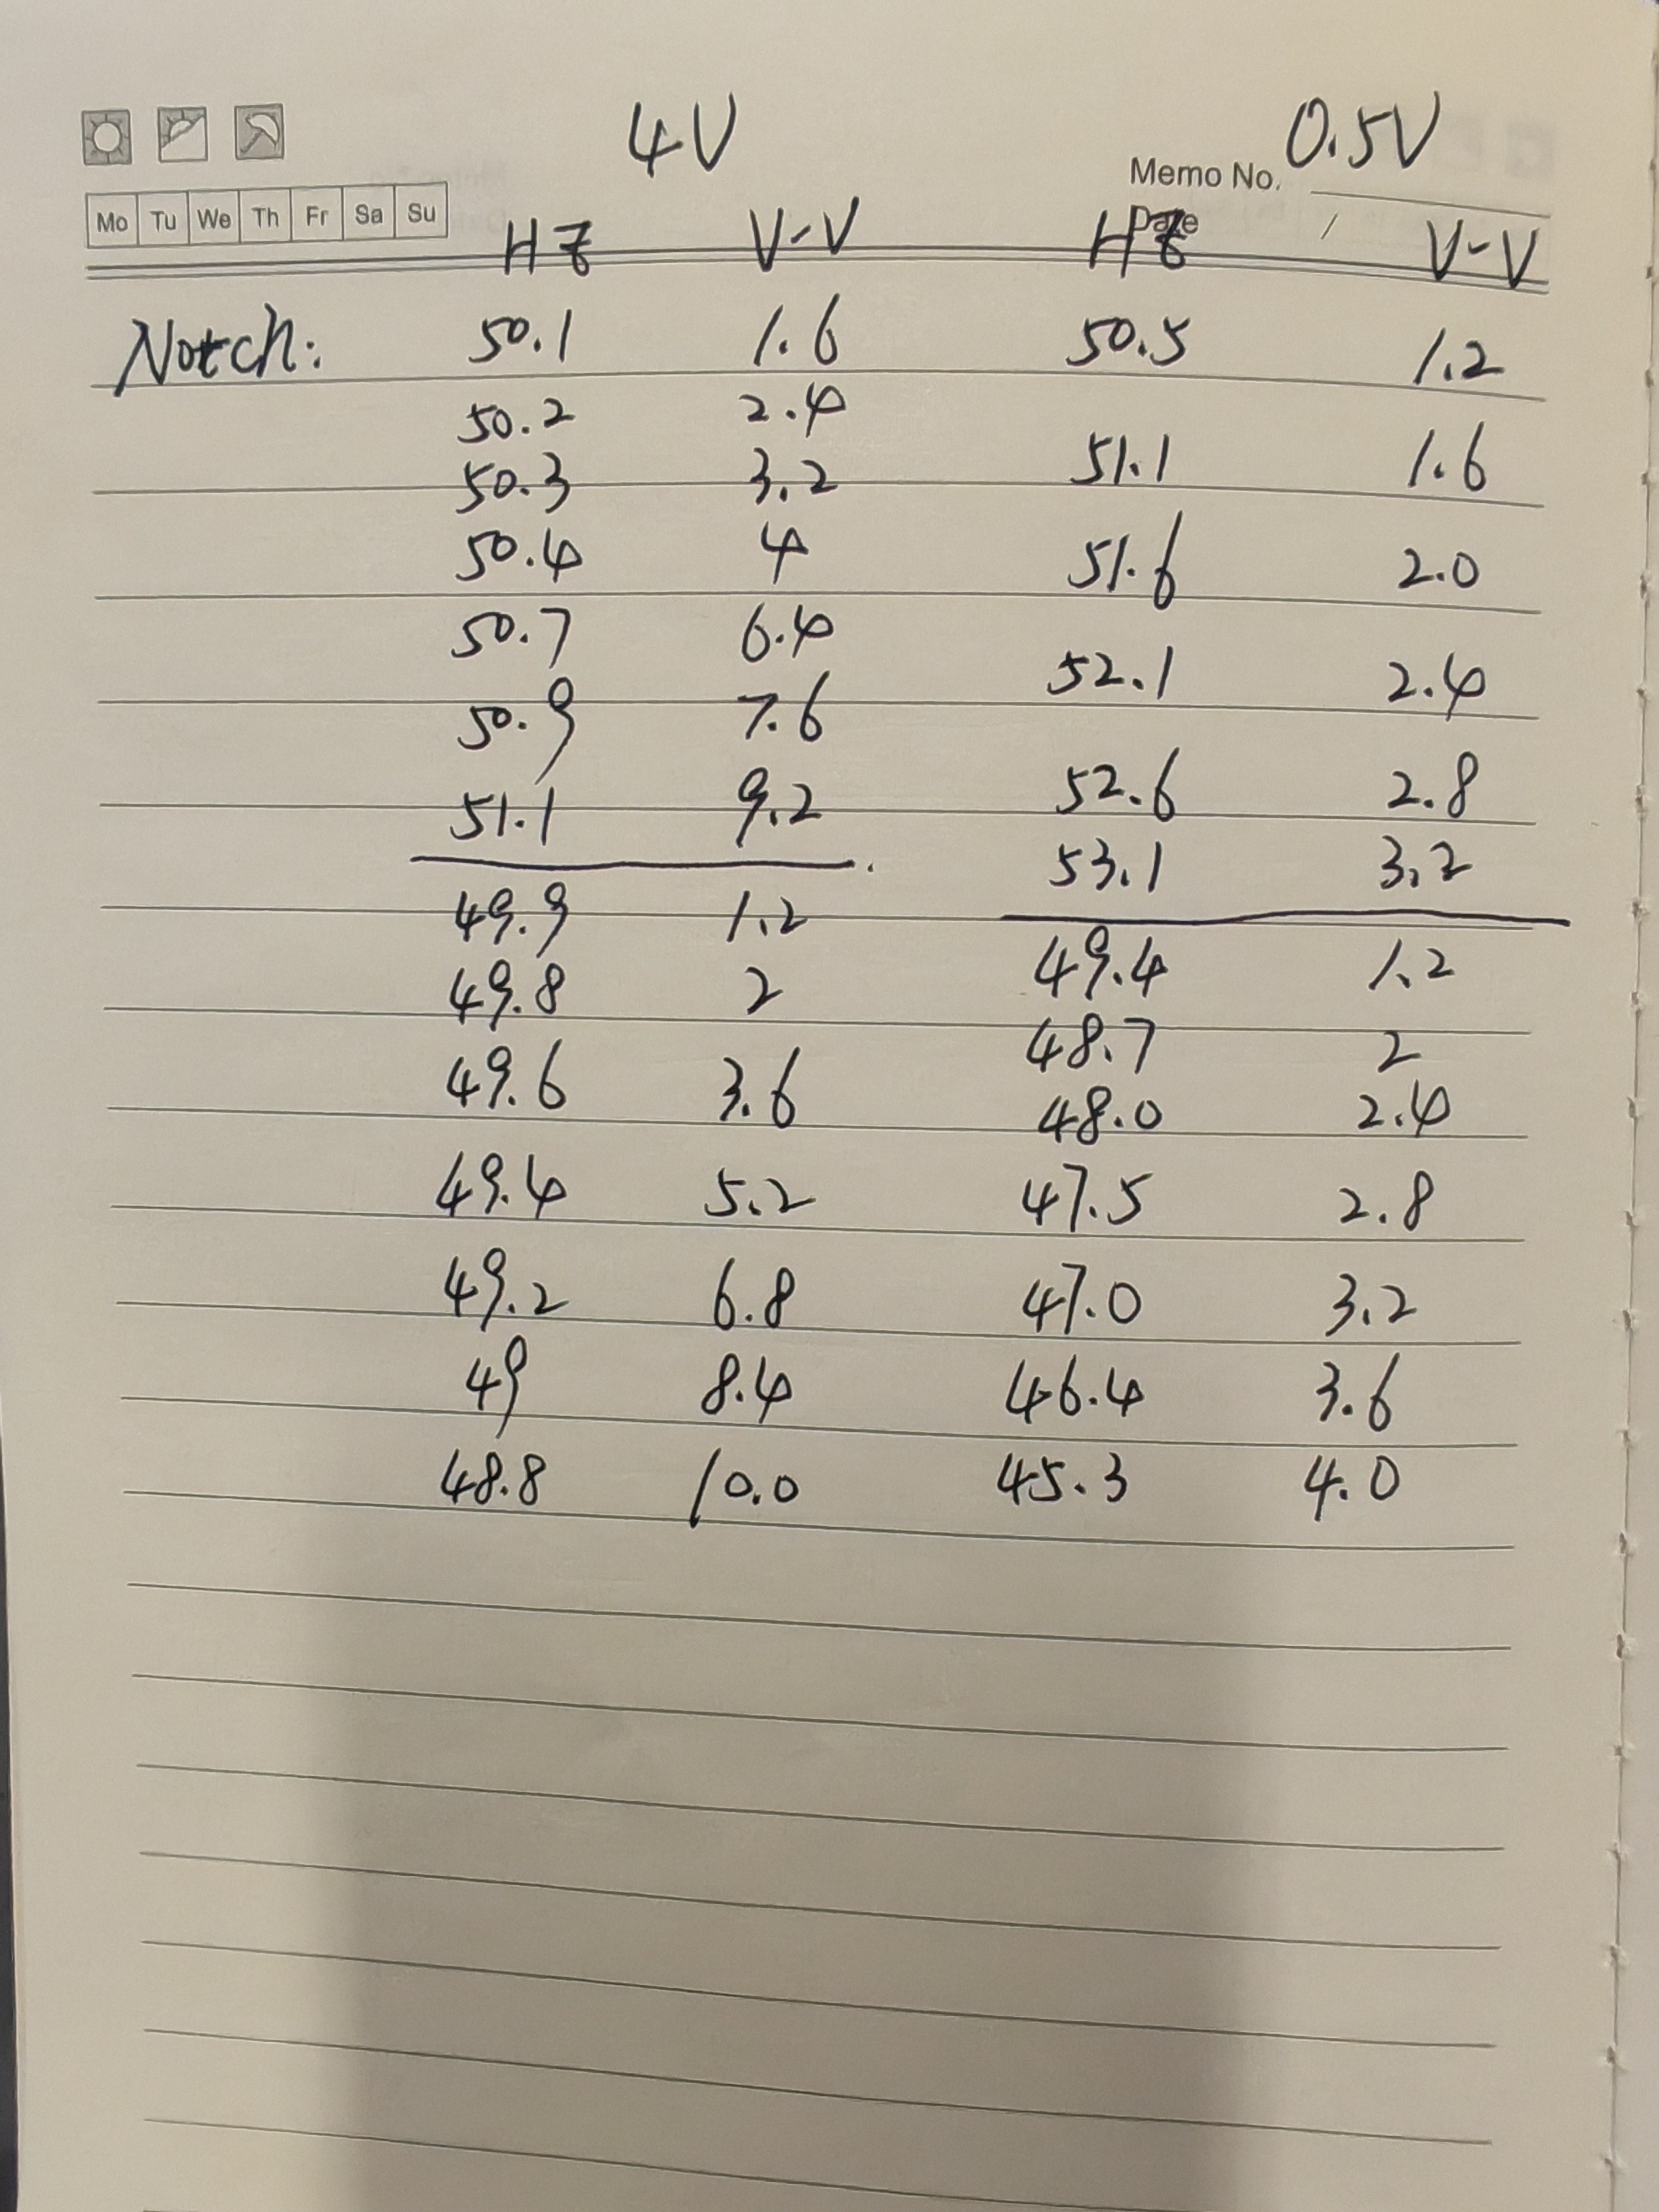
\includegraphics[width=200pt,height=350pt]{4&0.5.jpg}
    \caption{幅频特性}
\end{figure}

\begin{table}[htbp]
    \centering
    \caption{50Hz陷波器的幅频特性}
    \label{tab:example}

    \begin{tabular}{ccc}
    \hline 
    % 表头
    输入电压(V) & 频率(Hz) & 输出峰峰值(V-V) \\ 
    4 & 50.1 & 1.6 \\ 
    4 & 50.2 & 2.4 \\ 
    4 & 50.3 & 3.2 \\ 
    4 & 50.4 & 4.0 \\ 
    4 & 50.7 & 6.4 \\ 
    4 & 50.9 & 7.6 \\ 
    4 & 51.1 & 9.2 \\ 
    4 & 49.9 & 1.2 \\ 
    4 & 49.8 & 2.0 \\ 
    4 & 49.6 & 3.6 \\ 
    4 & 49.4 & 5.2 \\ 
    4 & 49.2 & 6.8 \\ 
    4 & 49 & 8.4 \\ 
    4 & 48.8 & 10.0 \\ 

    0.5 & 50.5 & 1.2 \\ 
    0.5 & 51.1 & 1.6 \\ 
    0.5 & 51.6 & 2.0 \\ 
    0.5 & 52.1 & 2.4 \\ 
    0.5 & 52.6 & 2.8 \\ 
    0.5 & 53.1 & 3.2 \\ 
    0.5 & 49.4 & 1.2 \\ 
    0.5 & 48.7 & 2.0 \\ 
    0.5 & 48.0 & 2.4 \\ 
    0.5 & 47.5 & 2.8 \\ 
    0.5 & 47.0 & 3.2 \\ 
    0.5 & 46.4 & 3.6 \\ 
    0.5 & 45.3 & 4.0 \\ 

\end{tabular}
    
\end{table}
\clearpage
\begin{tikzpicture}
    \begin{axis}[
        title=50Hz陷波器的幅频特性,
        xlabel=频率(Hz),
        ylabel=输出峰峰值,
        legend pos=north west
    ]
    % 直接从表格数据绘制
    \addplot table {
        x   y
        48.8  10.0 
        49  8.4 
        49.2  6.8 
        49.4  5.2
        49.6  3.6
        49.8  2.0
        49.9  1.2
         50.1  1.6 
         50.2  2.4 
         50.3  3.2 
         50.4  4.0 
         50.7  6.4 
         50.9  7.6 
         51.1  9.2     
    };
    \addlegendentry{$V_\text{in}$ = 4V}

    \addplot table {
        x   y
        45.3  4.0
        46.4  3.6
        47.0  3.2
        47.5  2.8
        48.0  2.4
        48.7  2.0 
        49.4  1.2  
        50.5  1.2 
        51.1  1.6  
        51.6  2.0  
        52.1  2.4  
        52.6  2.8  
        53.1  3.2  
           
    };
    \addlegendentry{$V_\text{in}$ = 0.5V}

    \end{axis}
    \end{tikzpicture}

相频特性记录如图:
\begin{figure}[htbp]
    \centering
    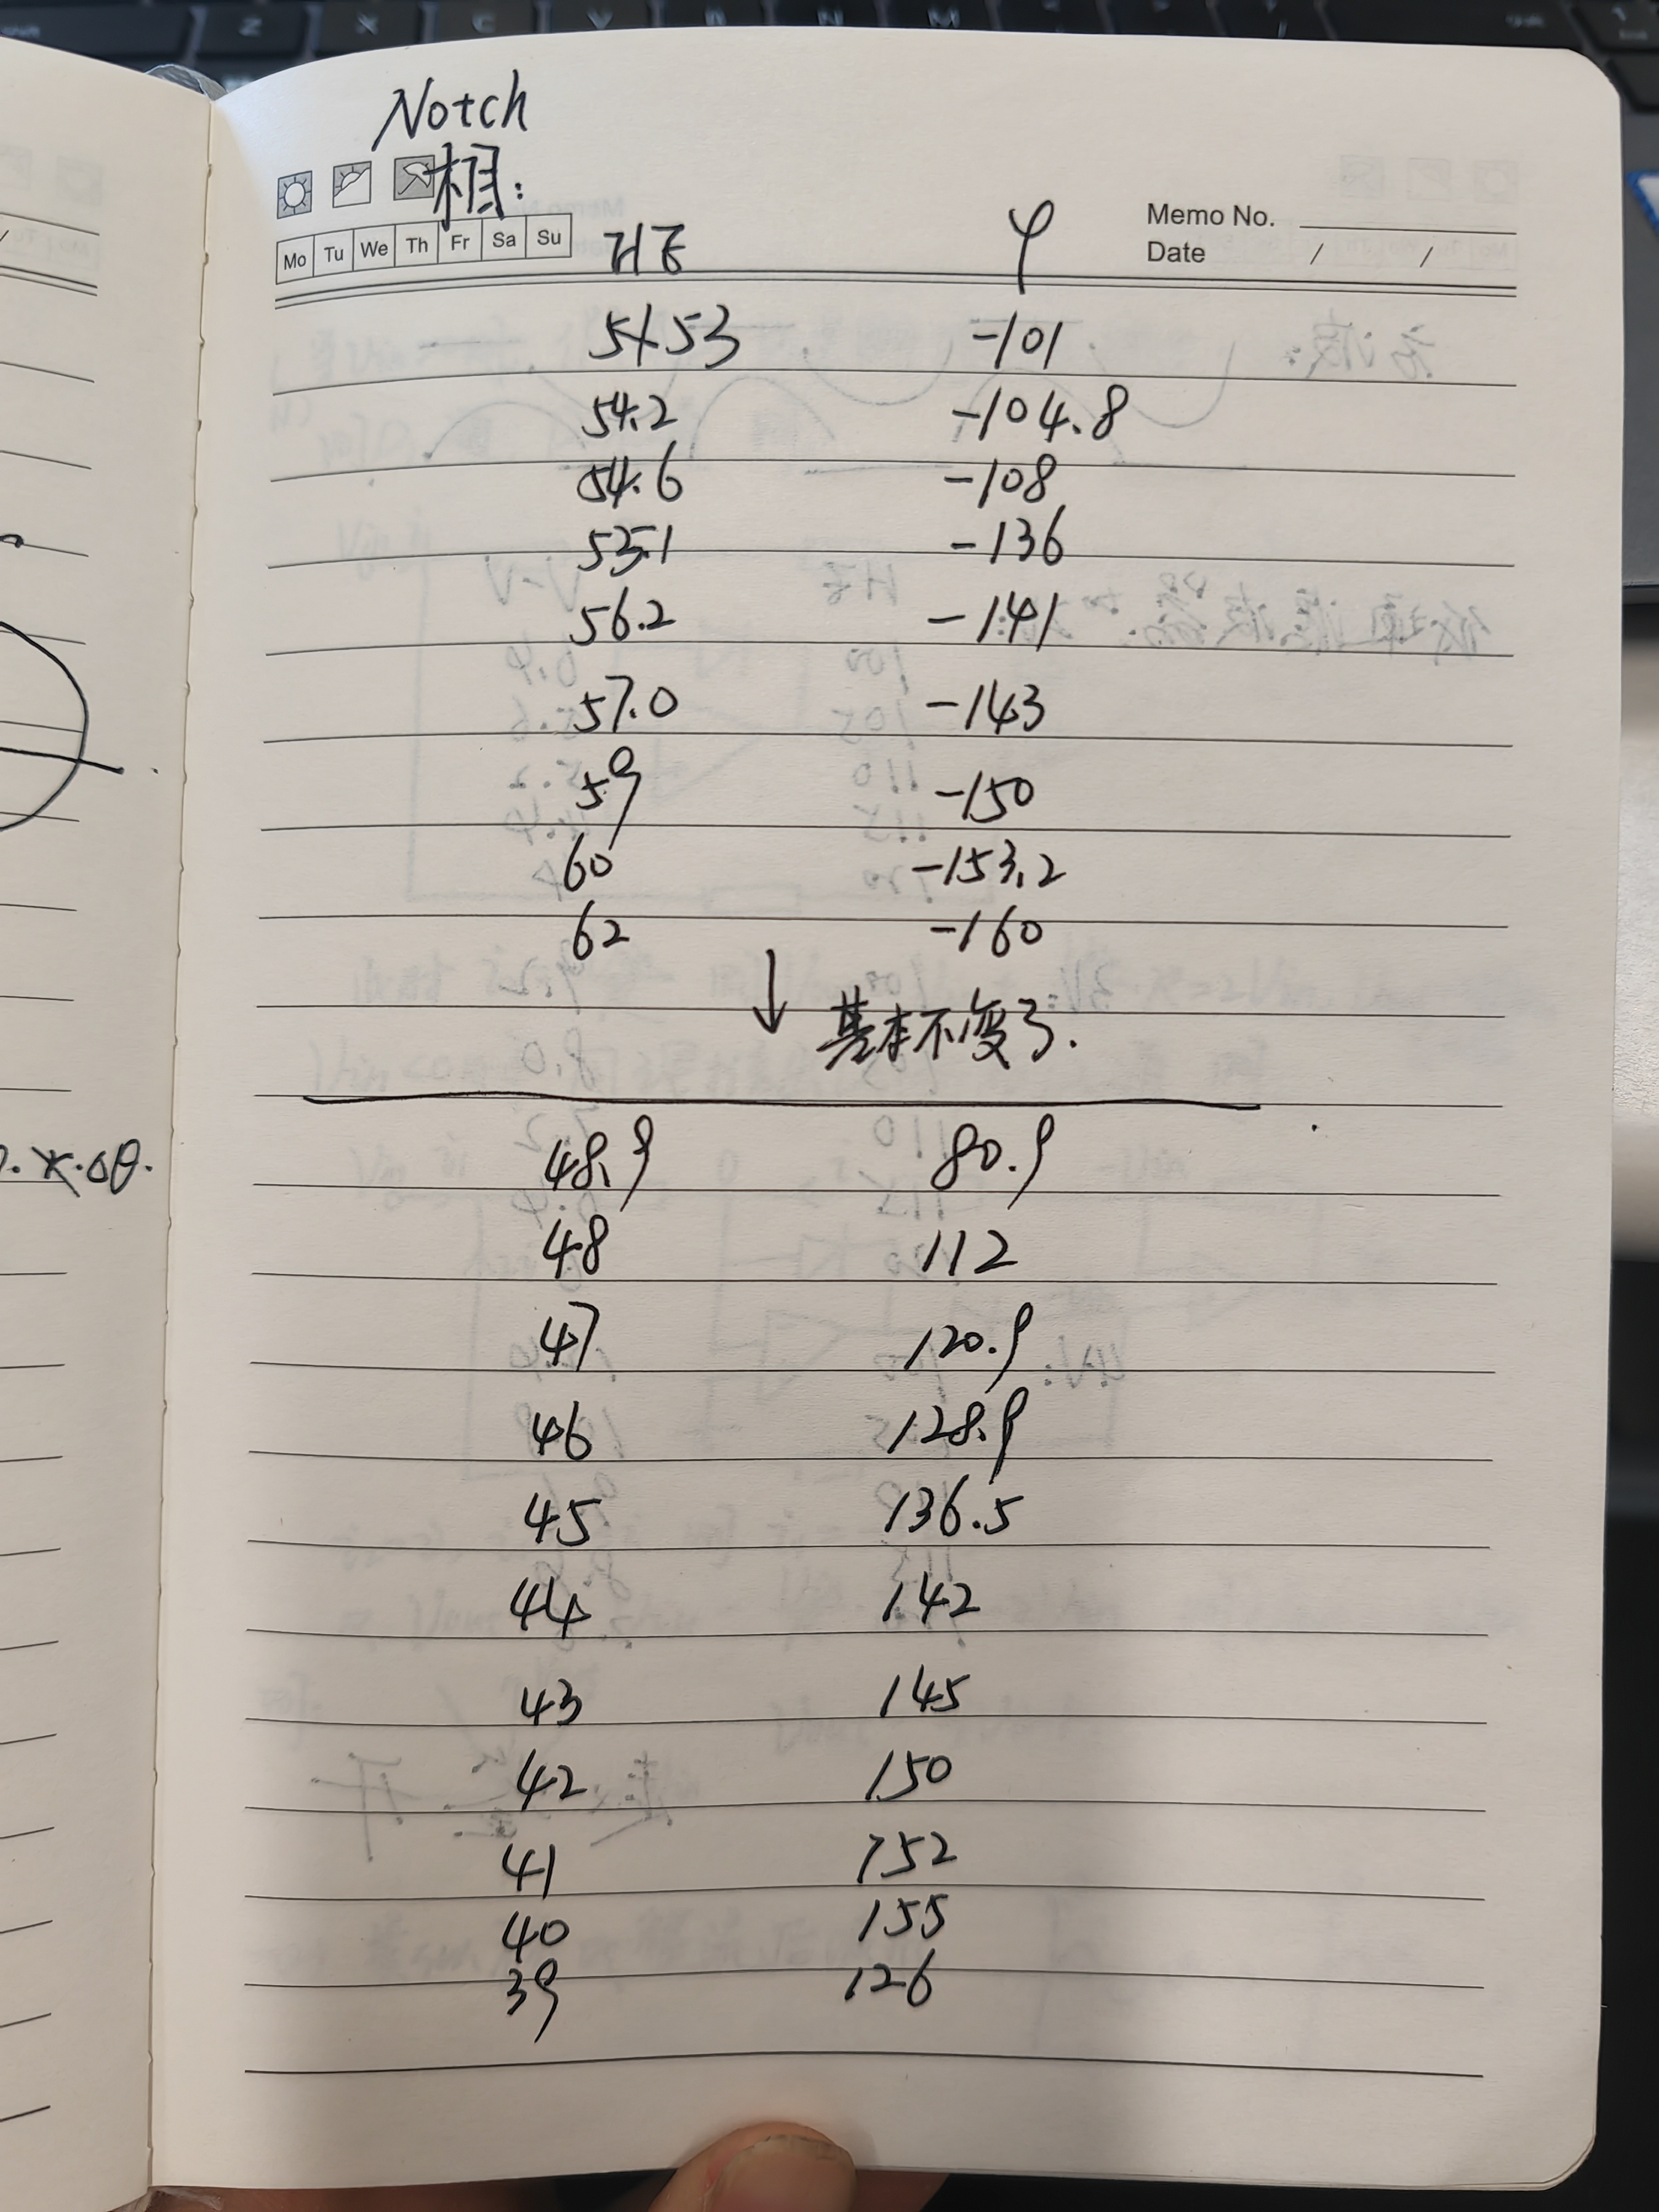
\includegraphics[width=300pt,height=220pt]{2V Norch.jpg}
    \caption{相频特性}
\end{figure}

\begin{table}[h!]
    \centering
    \caption{50Hz陷波器的相频特性(将负相位调整为正相位)}
    \label{tab:example}

    \begin{tabular}{cc}
    \hline 
    % 表头
    频率(Hz) & 相位$\phi$(°) \\ 
    53 & 79 \\ 
    54.2 & 75.2 \\
    54.6 & 72 \\ 
    55.1 & 44 \\ 
    56.2 & 39 \\ 
    57.0 & 37 \\ 
    59 & 30 \\ 
    60 & 27.8 \\ 
    62 & 20 \\ 
    48.9 & 80.9 \\
    48.0 & 112 \\
    47.0 & 120.9 \\
    46.0 & 128.9 \\
    45.0 & 136.5 \\
    44.0 & 142 \\
    43.0 & 145 \\
    42.0 & 150 \\
    41.0 & 152 \\
    40.0 & 155 \\
    39.0 & 126 \\
\end{tabular}
    
    \end{table}

    \begin{tikzpicture}
        \begin{axis}[
            title=50Hz陷波器的相频特性,
            xlabel=频率(Hz),
            ylabel=相位$\phi$(°),
            legend pos=north west
        ]
        % 直接从表格数据绘制
        \addplot table {
            x   y
            39.0  126 
            40.0  155 
            41.0  152 
            42.0  150 
            43.0  145 
            44.0  142 
            45.0  136.5 
            46.0  128.9 
            47.0  120.9 
            48.0  112 
            48.9  80.9 
            53  79  
            54.2  75.2 
            54.6  72  
            55.1  44  
            56.2  39  
            57.0  37  
            59  30  
            60  27.8  
            62  20 
        };
        \addlegendentry{$V_\text{in}$ = 2V}
        
        \end{axis}
        \end{tikzpicture}

\subsection{级联电路,观察并记录心电波形。记录心率,并折算原始心电信号的幅度}
心电波形如图所示:
\begin{figure}[htbp]
    \centering
    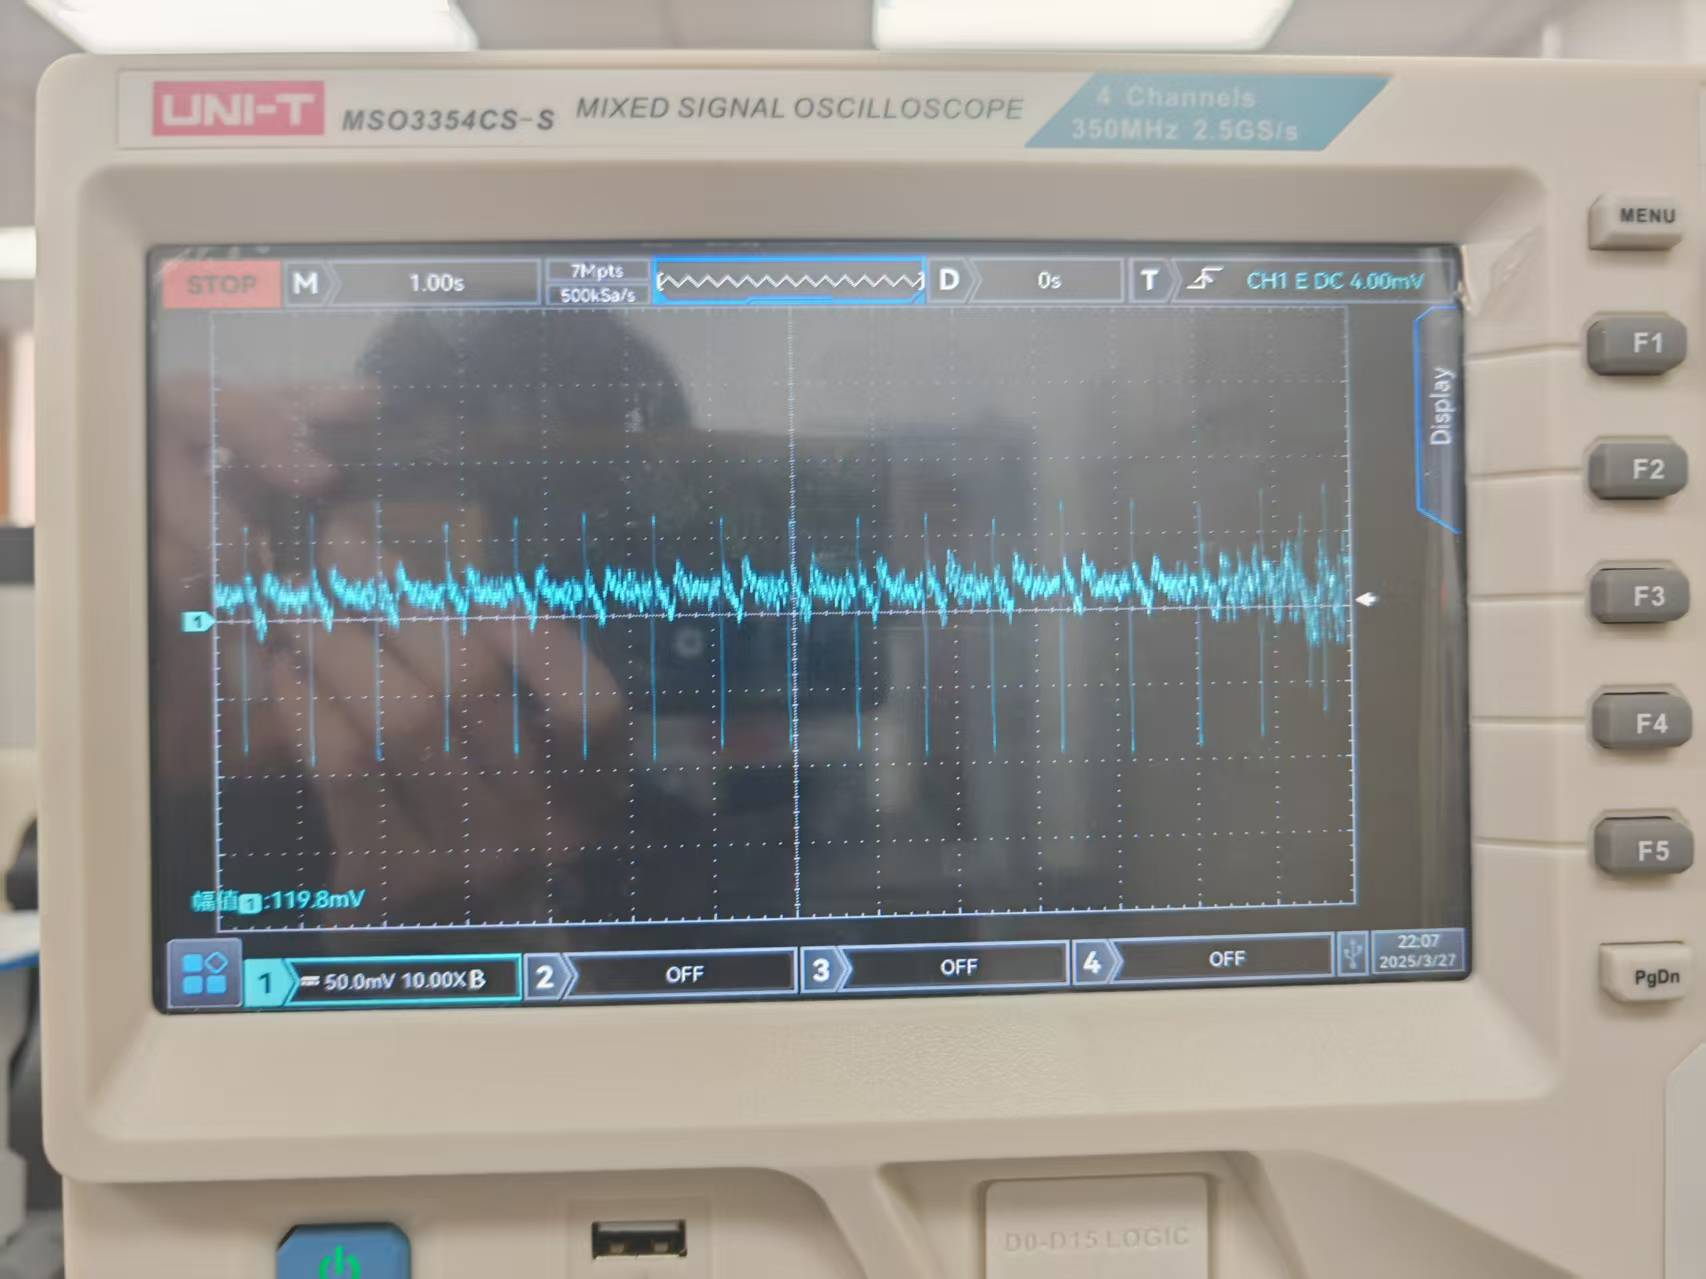
\includegraphics[width=300pt,height=220pt]{heart.jpg}
    \caption{心电波形}
\end{figure}
由此知峰峰值为119.8mV,峰极值为59.9mV,在被差分放大器放大前原始信号幅值为5mV左右。频率为1.19Hz,每分钟72下左右。

\section{实验总结}
\subsection{总结示波器(DSO-X2012A)、函数信号发生器(33210A)的正确使用方法}
\begin{enumerate}
    \item 开机
    \item 通道选择:按 Channel 1 或 Channel 2 激活对应通道,调节 Volts/Div 调整垂直灵敏度。
    \item 时基调节:使用 Time/Div 旋钮调整水平时间刻度,使信号波形清晰显示。
    \item 触发设置:选择合适的触发模式(如边沿触发),设置触发电平和触发源(如 CH1)。
    \item 使用 Measure 功能自动测量幅值、频率、周期等参数。
\end{enumerate}
\subsection{总结示波器测量各种时域波形参数和电路参数的方法}
\begin{enumerate}
    \item 开机
    \item 波形选择:按 Waveform 选择正弦波、方波、三角波等。
    \item 频率设置:通过数字键盘或旋钮输入目标频率(如 50Hz)。
    \item 幅值调节:按 Amplitude 设置输出电压(如 1Vpp)。
    \item 偏置调节:按 Offset 调整直流偏置(如 0V)。
    \item 按 Output On/Off 开启或关闭信号输出。
\end{enumerate}
操作过程中要注意接线最好不要碰在一块,防止短路,要有规划,不然调整一根线都要把几根线拆下来重装。

\section{思考题解答}
\subsection{为什么测量电路的频率响应时,要采用正弦信号进行激励?如果两个线性电路的幅频响应和相频响应均一致,能否认为这两个电路就是完全等效的电路?}
采用正弦信号的原因:
正弦信号是单一频率的信号,可以直观地反映电路对特定频率的响应特性。通过测量不同频率下正弦信号的幅度和相位变化,可以准确绘制电路的幅频特性和相频特性曲线。此外,正弦信号是线性时不变系统的基本激励信号,其输出仍然是同频率的正弦信号,便于分析和计算。
\\
完全等效的条件:
如果两个线性电路的幅频响应和相频响应均一致,只能说明它们在频域上的特性完全相同(即传递函数相同)。然而,电路的其他特性(如输入阻抗、输出阻抗、噪声性能、非线性失真等)可能不同。因此,不能仅凭幅频和相频响应一致就认为两个电路完全等效,还需要考虑其他参数是否一致。
\subsection{图中各电路模块的次序是否可以交换?为什么?}
各电路模块的次序通常不能随意交换,原因如下:
\\
差分放大器(仪表放大器):必须作为第一级,因为心电信号微弱且伴随高共模干扰,仪表放大器的高输入阻抗和高共模抑制比可以有效提取差模信号并抑制干扰。
\\
高通滤波器:应位于放大器之后,用于去除基线漂移和低频噪声(如呼吸干扰)。若放在放大器之前,可能因信号幅度过小而无法有效滤波。
\\
低通滤波器:用于滤除高频噪声,应放在高通滤波器之后,避免高频噪声干扰后续处理。
\\
50Hz陷波器:专门用于滤除工频干扰,通常放在信号链的中间或靠后位置,确保其他噪声已被初步滤除后再处理工频干扰。
\subsection{要实现对特定频率有较大衰减量的陷波器对元器件的精度有比较高的要求,在本实验中,通过测试并调节可变元件实现精密调节。在实际生产中,处于可靠性和成本的要求,
有的时候不允许使用可调元件,这时有下面两种常见的做法:}
\subsubsection{很多情况下,我们只关心两个电子元件的比值关系的精确性,而对绝对值的精确性要求不高。比如我们使用两个电阻构建一个分压比为1/2的精密分压器,只要求两个电阻的阻值相等就好。现有UT39A型万用表,一包(1000只)1\% 精度的100kΩ、1/4瓦电阻,和一个0~30V电压可调的电源,希望从中挑选出阻值相差0.1\% 或以下的两个电阻以构建此分压器。请问是否可能?如果可能,请描述实现方案。}
可能。根据抽屉原理可知,先取10个电阻测量,最坏情况为每个电阻彼此之间组阻值相差均大于等于0.1\%,但是由于整体误差最多只有1\%,那么第十一个的阻值一定和前十个中任意一个阻值差距小于0.1\% 。最多取11个即可至少有两个电阻符合要求。
\subsubsection{一般的薄膜电容的精度都在5\% 左右,图7是一种CB14型高精度电容,其精度可以达到0.5\% 。通过观察,可以发现这种电容是由两个电容体并联构成的,请分析为什么要这样做?图7高精度CB14聚苯乙烯电容}
理由如下:
\begin{enumerate}
    \item 提高精度:两个电容体并联后,总容值为两者之和。若单个电容的误差随机分布,并联可部分抵消误差,提高整体精度。
    \item 降低温度系数影响:不同电容体的温度特性可能互补,并联后整体温度稳定性更好。
    \item 冗余设计:若一个电容体失效,另一个仍能维持部分功能,提高可靠性。
\end{enumerate}
\end{document}